\section{}
\textit{
The diagram models a gate valve which regulates the fluid flow in an engine. The gate valve is
modelled as a pendulum (with a massless rod and uniform disk of mass $m$ and radius $r$) pinned
to the engine at $R$, and is controlled by a spring/damper mechanism connecting the centre of the
disk to the engine.}

\textit{
    The engine's motion during operation is denoted as $y = A \sin (\omega t)$ , and the distance from $R$
    to the centre of the disk is $a$. Assuming small oscillations, the total horizontal displacement of
    the disk is denoted as $x$. The relative motion $z(t)$ between the gate and engine is given as:}
\[z = x - y = a\theta\]
\textit{Note: the disk is fixed to the rod, so it does not spin about the point of connection with the rod,
but the rod itself is pinned at $R$. For a uniform disk, $J = \frac{1}{2} m r^2$.}

\begin{figure}[H]
    \centering
    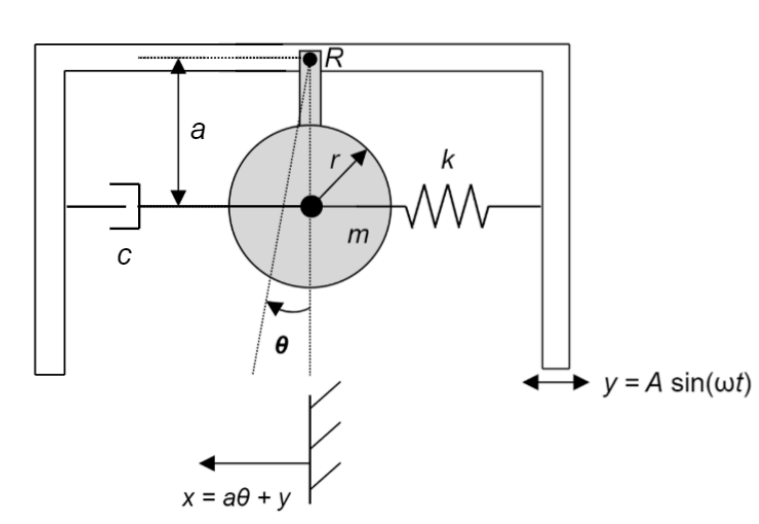
\includegraphics[width=0.5\linewidth]{Questions/Figures/Q1 Problem Diagram.png}
\end{figure}

\begin{enumerate}[label=(\alph*)]
    \item \textit{Determine the equation of motion for the relative motion of the gate with respect
    to the engine $z$, in terms of $m$, $k$, $a$, $g$, and $r$. Assume small oscillations.}
    \item \textit{If $\omega = 2400$ rpm, $a = 70$ mm, $r = 35$ mm, $m = 2.25$ kg, $k = 8.75$ kN/m, and
    $c = 30$ Ns/m, determine the amplitude of the relative motion $Z$ between the gate valve
    and engine in terms of $A$.}
\end{enumerate}

\subsection*{Solution}
\subsection{}
Here is the FBD and MAD for the problem:
\begin{figure}[H]
    \centering
    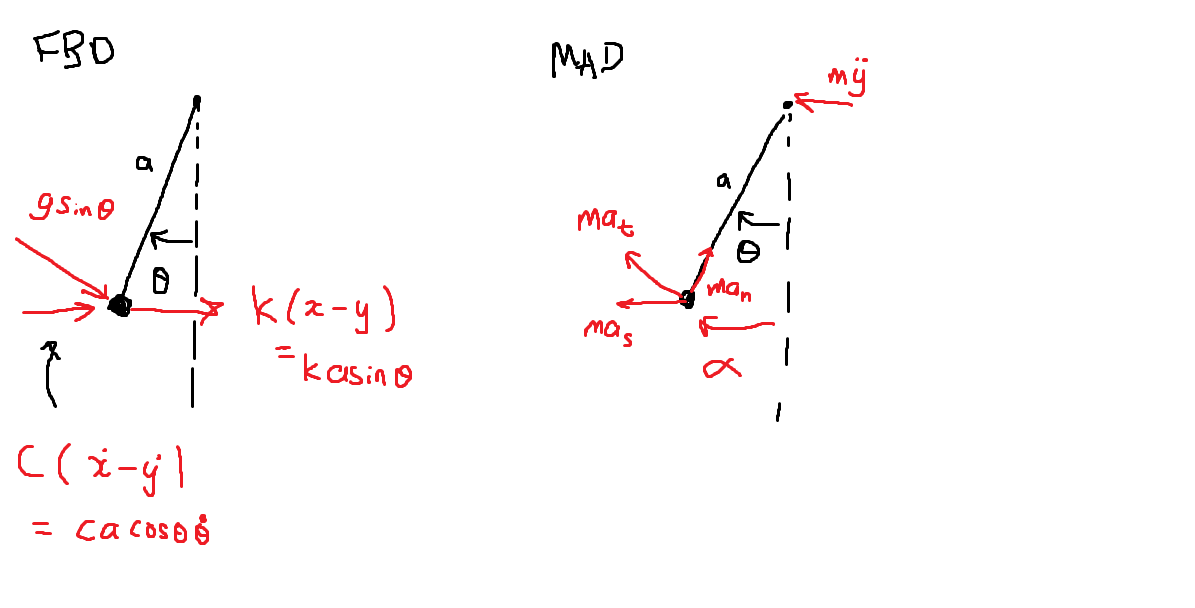
\includegraphics[width=0.8\linewidth]{Questions/Figures/Q1 FBD MAD.png}
\end{figure}

The equation of motion for the relative motion of the gate can be found by first taking the moment about the pin, $R$. Since the disk is undergoing rotation and translation, we consider general plane motion. First simplify the kinetic moment about the pin using the MAD diagram,
\begin{align}
    \circlearrowright \sum M_R &= (\mathcal{M}_k)_R \nonumber \\
    &= J_G \ddot{\theta}  + (a) m (a_G)_t  + (a \cos\theta) m (a_G)_s  \nonumber \\
    &= J_G \ddot{\theta} + ma (a\ddot{\theta})  + m(a \cos\theta) (\ddot{y})  \nonumber \\
    &= \underbrace{(J_G + m a^2)}_{J_{R}} \ddot{\theta} + m a \ddot{y} \cos\theta \label{eq:kinetic_moment}
\end{align}
Next, summing the moments in the FBD,
\begin{align}
    \circlearrowright \sum M_R &= -k a^2 \sin\theta - c a^2 \cos\theta \dot{\theta} - m g a \sin\theta \label{eq:force_moment}
\end{align}
Equating (\ref{eq:kinetic_moment}) and (\ref{eq:force_moment}), 
\begin{align*}
    J_R \ddot{\theta} + m a \ddot{y} \cos\theta &= -k a^2 \sin\theta - c a^2 \cos\theta \dot{\theta} - m g a \sin\theta
\end{align*}
Assuming small oscillations, we can use the small angle approximation, $\sin\theta \approx \theta$ and $\cos\theta \approx 1$ to simplify the equation.
\begin{align*}
    J_R \ddot{\theta} + m a \ddot{y} &= -k a^2 \theta - c a^2 \dot{\theta} - m g a \theta
\end{align*}
Rearranging,
\begin{align*}
    \left[J_R \right] \ddot{\theta} + \left[c a^2 \right] \dot{\theta} + \left[ k a^2 + m g a \right] \theta &= - m a \ddot{y}
\end{align*}
Since $z = a\theta$, multiplying both sides by $a$,
\begin{align*}
    \left[J_R \right] a \ddot{\theta} + \left[c a^2 \right] a \dot{\theta} + \left[ k a^2 + m g a \right] a \theta &= - m a^2 \ddot{y} \\
    \left[J_R \right] a z + \left[c a^2 \right] \dot{z} + \left[ k a^2 + m g a \right] z &= - m a^2 \ddot{y} 
\end{align*}
Finally,
\begin{align*}
    \Aboxed{\underbrace{\left[\frac{1}{2} m r^2 + m a^2 \right]}_{m_{\text{eff}}} \ddot{z} + \underbrace{\left[c a^2 \right]}_{c_{\text{eff}}} \dot{z} + \underbrace{\left[ k a^2 + m g a \right]}_{k_{\text{eff}}} z &= \underbrace{m a^2 A \omega^2}_{F_o} \sin(\omega t)}
\end{align*}

\subsection{}
This is the standard form of a forced, damped harmonic oscillator. From Eq. (5.9) in the textbook, the amplitude is 
\begin{align*}
    \mathbb{X} &= \frac{F_o}{\sqrt{\left(k_{\text{eff}} - m_{\text{eff}} \omega^2 \right)^2 + \left(c_{\text{eff}} \omega \right)^2}}
\end{align*}
Determining the effective mass, damping, and stiffness,
\begin{align*}
    m_{\text{eff}} &= \frac{1}{2} m r^2 + m a^2 = \frac{1}{2} (2.25)(0.035)^2 + (2.25)(0.070)^2 = 0.0124 \\
    c_{\text{eff}} &= c a^2 = (30)(0.070)^2 = 0.147 \\
    k_{\text{eff}} &= k a^2 + m g a = (8.75)(0.070)^2 + (2.25)(9.81)(0.070) = 1.58795 \\
    F_o &= m a^2 A \omega^2 = (2.25)(0.070)^2 (2400 \times 2\pi / 60)^2 A= 696.3993 A
\end{align*}
Substituting into the amplitude equation,
\begin{align*}
    \mathbb{X} &= \frac{696.3993}{\sqrt{\left(1.58795 - 0.0124 (2400 \times 2\pi / 60)^2 \right)^2 + \left(0.147 (2400 \times 2\pi / 60) \right)^2}} A \\
    &= \boxed{0.890 A}
\end{align*}